\documentclass[
headings=optiontohead,              % allows double headers
12pt,                               % fontsize 
DIV=13,                             % koma script diveider amount. tells koma how much of the site can be written to
twoside=false,                      % if set to true, automatically formats as book style with different left and right pages
open=right,                         % starting page on twosided texts 
BCOR=10mm,                          % correction that accounts for the center of the pages being glued in
toc=bibliographynumbered            % bibliography gets a number and is listed in the table of contents
]{scrreport}

\usepackage[utf8]{inputenc}                     % correct encoding of output, technically not needed anymore
\usepackage[T1]{fontenc}                        % correct encoding of output, technically not needed anymore
\usepackage[english]{babel}                     % font that supports English
\usepackage{upgreek}                            % non-cursive Greek letters
\usepackage[stretch=10,shrink=10,protrusion=true,expansion=true,final]{microtype} % prettier block format
\usepackage{hyperref}                           % links for everything
\usepackage{color}                              % allows for setting in different colors
\usepackage[autooneside=false,automark]{scrlayer-scrpage} % page-style with "Kolumnentitel" (title of current chapter is displayed at the top)
\usepackage{lmodern}                            % alternative font (better use libertinus)
\usepackage[sb]{libertinus}                     % use the font libertinus (needs to be installed from the web)
\usepackage[slantedGreek]{libertinust1math}     % math mode improvement for libertinus
\usepackage{siunitx}                            % physical units setting
\usepackage{icomma}                             % commas in lists get extra space if needed                        
\usepackage{amsfonts,amssymb,amstext,amsmath,amsthm} % better math mode (\mathrm and \text) and symbols
\usepackage{xspace}                             % works to improve own commands and provides "\xspace"-command, that puts a space if needed
\usepackage{ifthen}                             % more control over non-obligatory parameters
\usepackage{titling}                            % get title values as macros
\usepackage[onehalfspacing]{setspace}           % control the spacing between lines and in enumeration lists
\usepackage[backend=biber, style=phys, biblabel=brackets]{biblatex} % citations with "modern" backend and an physics-accepted citation style
\usepackage{graphicx}                           % work with graphics 
\usepackage{ragged2e}                           % ragged-commands (when no block format is wanted)
\usepackage{pdfpages}                           % allows including of pdfs into this pdf
\usepackage{booktabs}                           % better table formatting
\usepackage{multicol}                           % allows for the definition of multi-columns in tables
\usepackage{multirow}                           % allows for the definition of multirow-tables instead of just multicolumn
\usepackage{float}                              % provides the "H" option for forcing placement of a figure
\usepackage[section]{placeins}                  % provides the command "\FloatBarrier" to control the end of floatable regions for figures/tables
\usepackage{floatpag}                           % make it possible for float-pages to not have a page number
\usepackage{url}                                % sometimes needed by biblatex, technically no longer needed
\usepackage{minted}                             % nice code highlighting (needs Python Package to compile!!)
\usepackage{accents}                            % better control over accents
\usepackage{mathtools}                          % more math control possibilities
\usepackage[autostyle=true]{csquotes}           % context-sensitive-quotes -> quotation marks that are set correctly for the context
\usepackage{physics}                            % bra-ket and more

\title{Investigation of transformer architectures for geometrical graph structures and their application to two-dimensional spin systems} % TODO lookup title
\author{Jonas Kell}
\date{7$^\text{th}$ October 2022}

\input{config}                                  % another file that holds the package/document configuration
\input{format}                                  % another file that holds format information
%! Ref-Commands 
\newcommand*{\fullref}[1]{\hyperref[{#1}]{\textit{\autoref*{#1} \nameref*{#1}}}}
\newcommand*{\fullpage}[1]{\hyperref[{#1}]{Seite \pageref*{#1}}}
\newcommand*{\fullpages}[1]{\hyperref[{#1}]{Seiten \pageref*{#1}ff}}

%! Math operators and other small conveniences
\newcommand\thickbar[1]{\accentset{\rule{.6em}{.8pt}}{#1}}
\DeclareMathOperator{\ggt}{ggT}
\DeclareMathOperator{\kgv}{kgV}
\DeclarePairedDelimiter\ceil{\lceil}{\rceil}
\DeclarePairedDelimiter\floor{\lfloor}{\rfloor}
                                % another file that holds predefined commands


\begin{document}

% ! Bibliography, page numbering and Title setups
\thispagestyle{empty}                           % make sure title page is not numbered or anything else


\newcommand{\mail}{jonas.kell@student.uni-augsburg.de}



\begin{titlepage}
\makebox[\textwidth][c]{\includegraphics[width=0.5\textwidth]{logo_uni_augsburg.jpg}}
    
\color{dblue}

\begin{center}
    \vspace*{2cm}
    \Huge
    \textbf{\thetitle}

    \vspace*{1.5cm}
    \color{black}
    \textbf{Bachelor Thesis}

    \vspace*{1cm}
    \normalsize
    submitted by\\
    \LARGE
    \theauthor\\\vspace*{0.3cm}
    \normalsize
    on \thedate

    \vspace{1.8cm}
    \color{black}
    \emph{Augsburg University}\\
    \emph{Faculty of Applied Computer Science}\\
    \emph{Institute of Computer Science}\\
    \emph{Chair for Machine Learning \& Computer Vision}

    \vfill

    \begin{tabular}{rl}
        1$^\text{st}$ Corrector: &Prof. Dr. Rainer Lienhart\\
        2$^\text{nd}$ Corrector: &Prof. Dr. Markus Heyl\\
    \end{tabular}
\end{center}

\end{titlepage}
                               % include title-page
\cleardoublepage                                % make sure, that if double-page is active, to reset the double page counter
\pagestyle{scrheadings}                         % puts current chapters title into the header in small gray font
\pagenumbering{roman}                           % number the pages of the table of contents in roman numerals
\renewcommand{\contentsname}{Table of Contents} % title of table of contents
\tableofcontents                                % table of contents
\noindent\\\\

\addsec*{List of Abbreviations}
\begin{tabular}[h]{p{3cm}|l}
	Abbreviation & Meaning\\
	\hline
	AI & artificial intelligence\\ 
	NQS & Neural Quantum State\\
	VMC & Variational Monte Carlo\\
	DMC & Diffusion Monte Carlo\\
	nn & nearest neighbor\\
	nnn & next nearest neighbor\\
	sgd & stochastic gradient descent\\
	GPU & graphics processing unit\\
	ReLU & rectifier linear unit\\
	RBM & restricted Boltzmann machine\\
	fcl & fully connected layer\\
	MLP & multi layer perceptron\\
	rgb & red green blue\\
	sdp attention & scaled dot product attention\\
	swin & shifted window\\
	XLA & Accelerated Linear Algebra\\
	pe & positional encoding\\
	sr & single real\\
	sc & single complex\\
	tr & two real\\
	spc & split complex\\
	NaN & Not a Number \\
\end{tabular}\\\\

The abbreviations of the different metaformer names are collected in \autoref{table:metaformer-names}.

\newpage                                   % list of abbreviations, figures, etc
\cleardoublepage                                % make sure, that if double-page is active, to reset the double page counter
\pagenumbering{arabic}                          % number the pages of the main document in Arabic numerals

% After this, the redefinition of the "Kolumnentitel" takes place
\clearpairofpagestyles
\ihead{\leftmark}
\ohead{\Ifstr{\leftmark}{\rightmark}{}{\rightmark}}
\cfoot*{\pagemark}
% End of the "Kolumnentitel" redefinition


% ! Main Document Body
\chapter{Introduction}
\label{sec:introduction}
% TODO

% SOURCE: \cite{pytorchGithub}
% SOURCE: \cite{dinoGithub}
% SOURCE: \cite{einopsGithub}
% SOURCE: \cite{positionalEncodingGithub}
% SOURCE: \cite{poolformerGithub}

\FloatBarrier
\chapter{Theory}
\label{sec:theory}
    \section{From the Point of Physics}
        \label{sec:theory-physics}
        % TODO

% SOURCE: \cite{pytorchGithub}
% SOURCE: \cite{dinoGithub}
% SOURCE: \cite{einopsGithub}
% SOURCE: \cite{positionalEncodingGithub}
% SOURCE: \cite{poolformerGithub}

        \FloatBarrier
        \subsection{The Ground State Search}
        \label{sec:theory-groundstatesearch}
        This section is supposed to introduce the fundamentals of (many body) quantum physics.


        \subsection{The Ising Model}
        \label{sec:theory-ising}
        The model was first solved for a 1D chain by Ernst Ising in 1924 \cite*[]{isingFerromagnetismn}
        \FloatBarrier
        \subsection{Numerical Solution}
        \label{sec:theory-numericalsolution}
        With the combined knowledge of the two last sections, the ground state (and the ground state energy) can be calculated. It will become evident, that the calculation is really simple to do and program. Sadly it won't be feasable to compute sufficiently large lattices, because of the exponential nature of the problem.

\begin{figure}[htbp]
    \centering
    \makebox[\textwidth][c]{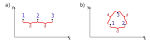
\includegraphics[width=0.9\textwidth]{./theory/physics/numerical-solutions/simple_case.pdf}}
    \vspace{-1.5cm}
    \caption{A representation of two simple latices. The spins are fixed at the point of the numbered locations. All sites have the same distance $d$ from each other. Note, that a spin up \up is directed parallel to the z-axis. That means in this case it would point out of the paper in the direction of the viewer.}
    \label{fig:simpleThreeLatticeIsing}
\end{figure}

In the beginning one trivial example will be discussed. The lattice is visualized in \autoref{fig:simpleThreeLatticeIsing}, image a).
This corresponds to a linear lattice in 1D. Let the Hamiltonian be the one in \ref{eq:hamiltonianExampleA}.

\begin{equation}
    \label{eq:hamiltonianExampleA}
    \hamiltonian = \sigma^z_1\sigma^z_2 + \sigma^z_2\sigma^z_3
\end{equation}

This hamiltonian is anti-ferromagnetic ($J = +1$). It should be easily seen, that the Energy $E$ in \ref{eq:schroedinger-general} becomes minimal (largest magnitude with negative sign) when the spins always point into the opposite direction as their neighbors: $\ket{\up, \down, \up}$ or $\ket{\down, \up, \down}$. This is quite a crucial step, so trying this by one self is advised for someone without prior quantum mechanical experience.
The ground state therefore will be a \emph{superposition} consisting of equal parts $\ket{\up, \down, \up}$ and $\ket{\down, \up, \down}$ \ref{eq:solutionSimpleExample}. The factor $\frac{1}{\sqrt[]{2}}$ instead of the seemingly more obvious $\frac{1}{2}$ makes the wavefunction be \emph{normalized}. If it wasn't for the square root, \autoref{eq:base-orthonormal} would not be satisfied. This way it is satisfied, which can be tested.

\begin{equation}
    \label{eq:solutionSimpleExample}
    \Psi_\mathrm{gnd} = \frac{1}{\sqrt[]{2}} \cdot \ket{\up, \down, \up} +  \frac{1}{\sqrt[]{2}} \cdot \ket{\down, \up, \down}
\end{equation}

The second example, visualized in \autoref{fig:simpleThreeLatticeIsing}, image b), however is not so simple. The corresponding hamiltonian can be seen in \ref{eq:hamiltonianExampleB}.
\begin{equation}
    \label{eq:hamiltonianExampleB}
    \hamiltonian = \sigma^z_1\sigma^z_2 +\sigma^z_2\sigma^z_3 +\sigma^z_1\sigma^z_3
\end{equation}
It has one more interaction than the previous one. Even though it also is anti-symmetric, it is \emph{not} possible to align all three spins in a way, so that they stand anti-parallel to all their neighbors. This phenomenon is called \emph{frustration} \cite*{frustration}.

Already this minimal problem has a complex superposition of eight base states as a ground state. The introduction of the transverse field will only make this more complex. Therefore a systematic way of finding the solution will be presented.

For this purpose, the example from \autoref{fig:simpleThreeLatticeIsing}, image b) will be used once more, but this time with the hamiltonian \ref{eq:hamiltonianExampleTransverse}.
\begin{equation}
    \label{eq:hamiltonianExampleTransverse}
    \hamiltonian = J\cdot \sigma^z_1\sigma^z_2 +J\cdot\sigma^z_2\sigma^z_3 +J\cdot\sigma^z_1\sigma^z_3
    +h \sigma^x_1+h \sigma^x_2+h \sigma^x_3
\end{equation}

The goal is now, to write the hamiltonian \hamiltonian as a matrix. 
The elements of the matrix should be $\bra{m}\hamiltonian\ket{n}$. Where $\ket{m}$ and $\ket{n}$ are two states out of the chosen basis. In this case the eight base states are the following:

\begin{center}
    \begin{tabular}{llll} 
        1: $\ket{\up, \up, \up}$ & 2: $\ket{\up, \up, \down}$  & 3: $\ket{\up, \down, \up}$  & 4: $\ket{\up, \down, \down}$ \\
        5: $\ket{\down, \up, \up}$ & 6: $\ket{\down, \up, \down}$  & 7: $\ket{\down, \down, \up}$  & 8: $\ket{\down, \down, \down}$ 
    \end{tabular}
\end{center}

In \ref{eq:matrixElement} an example calculation of $\bra{2}\hamiltonian\ket{4}$ is presented.

\begin{equation}
    \label{eq:matrixElement}
    \begin{split}
        &\bra{\up, \up, \down} \hamiltonian \ket{\up, \down, \down} = \\\\ % new line
         \bra{\up, \up, \down} J\cdot \sigma^z_1\sigma^z_2 \ket{\up, \down, \down} +
         &\bra{\up, \up, \down} J\cdot \sigma^z_2\sigma^z_3 \ket{\up, \down, \down} +
         \bra{\up, \up, \down} J\cdot \sigma^z_1\sigma^z_3 \ket{\up, \down, \down} +\\
         \bra{\up, \up, \down} h\cdot \sigma^x_1 \ket{\up, \down, \down} +
         &\bra{\up, \up, \down} h\cdot \sigma^x_2 \ket{\up, \down, \down} +
         \bra{\up, \up, \down} h\cdot \sigma^x_3 \ket{\up, \down, \down}\stackrel{\ref{eq:pauli-transformation}, \ref{eq:pauli-many-body}}{=}\\\\ % new line
          \bra{\up, \up, \down} J\cdot  1 \cdot (-1) \ket{\up, \down, \down} +
         & \bra{\up, \up, \down} J\cdot (-1) \cdot (-1) \ket{\up, \down, \down} +
          \bra{\up, \up, \down} J\cdot  1 \cdot (-1) \ket{\up, \down, \down} +\\
          \bra{\up, \up, \down} h\cdot  1 \cdot \ket{\down, \down, \down} +
         & \bra{\up, \up, \down} h\cdot 1 \cdot \ket{\up, \up, \down} +
          \bra{\up, \up, \down} h\cdot  1 \cdot \ket{\up, \down, \up} =\\\\ % new line
          (-J)\cdot      \bra{\up, \up, \down}  \ket{\up, \down, \down} +
         & J\cdot        \bra{\up, \up, \down} \ket{\up, \down, \down} +
          (-J)\cdot      \bra{\up, \up, \down}  \ket{\up, \down, \down} +\\
          h\cdot         \bra{\up, \up, \down}  \ket{\down, \down, \down} +
         & h\cdot        \bra{\up, \up, \down} \ket{\up, \up, \down} +
          h\cdot         \bra{\up, \up, \down}  \ket{\up, \down, \up}\stackrel{\ref{eq:base-orthonormal}}{=}\\\\ % new line
          (-J)\cdot 0 + J\cdot 0 &+  (-J)\cdot 0 + h\cdot 0  + h\cdot 1 + h\cdot 0   = h 
    \end{split}
\end{equation}
        \FloatBarrier
        \subsection{Solutions with Neural Quantum States}
        \label{sec:theory-neuralquantumstates}
        \subsection{Imaginary Time Evolution}
        \label{sec:theory-imagenarytimeevolution}
        \subsection{Explored Lattice Patterns}
        \label{sec:theory-latticepatterns}
    \section{From the Point of Computer Science}
        \label{sec:theory-cs}
        % TODO

% SOURCE: \cite{pytorchGithub}
% SOURCE: \cite{dinoGithub}
% SOURCE: \cite{einopsGithub}
% SOURCE: \cite{positionalEncodingGithub}
% SOURCE: \cite{poolformerGithub}

        \FloatBarrier
        \subsection{The Image Classification Task}
        \label{sec:theory-imageclassification}
        \subsection{Neural Network Training}
        \label{sec:theory-neuralnetworktraining}
        \subsection{Neural Network Pre-Training}
        \label{sec:theory-pretraining}
        \subsection{Employment of Graphs for Problem transfer}
        \label{sec:theory-graphs}

\chapter{Machine Learning Architectures}
\label{sec:architectures}

    \section{Used Architectures}
        \subsection{Perceptron Architectures}
        \label{sec:architectures-perceptron}
        \subsection{Pooling}
        \label{sec:architectures-pooling}
        \subsection{Convolutional Architectures}
        \label{sec:architectures-convolution}
        \subsection{Attention and the Transformer}
        \label{sec:architectures-attention}
        \subsection{The Metaformer}
        \label{sec:architectures-metaformer}
        \subsection{Graph Architectures}
        \label{sec:architectures-graphs}
    \section{Usage of Inductive Biases}
        \subsection{Conventional Architectures}
        \label{sec:architectures-biasesnormal}
        \subsection{Metaformer Architectures}
        \label{sec:architectures-biasesmetaformer}
        \subsection{Graph Architectures}
        \label{sec:architectures-biasesgraph}

\chapter{Experiments and their Results}
    \section{Metaformer in Image Classification}
        \subsection{Training Settings}
        \label{sec:experiments-trainingsettings}

        \subsection{Importance of Positional Encoding}
        \label{sec:experiments-positionalencoding}
        \subsection{Comparison of different Token Mixers}
        \label{sec:experiments-tokenmixers}

    \section{Metaformer in Ground State Search}
        \subsection{Comparison to established Architectures}
        \label{sec:experiments-comparisontoestablished}
        \subsection{Resiliency to the Choice of Lattice Encoding}
        \label{sec:experiments-resiliencylatticeencoding}
        \subsection{Optimizing the Ansatz}
        \label{sec:experiments-optimizingtheansatz}
        \subsection{Choice of Hyperparameters}
        \label{sec:experiments-hyperparameters}
        \subsection{Differences across the Phase Diagram}
        \label{sec:experiments-phasecriticalpoint}

\chapter{Conclusion}
\label{sec:conclusion}

% ! Addendum
\input{bibliography}
\chapter{Appendix}
\label{sec:appendix}

%! needs to be first, because of format adapted to chapter title of appendix
\section{Lattice Visualization} \label{appendix:lattice-visualisation}

\begin{minipage}{\linewidth}
    \centering
    \makebox[\textwidth][c]{
        \makebox[1.25\textwidth][c]{
            \makebox[0.40\textwidth][l]{\includegraphics[width=0.33\textwidth]{./../appendix/lattice_visualization/cubic,size=2,np.pdf}}
            \makebox[0.40\textwidth][l]{\includegraphics[width=0.33\textwidth]{./../appendix/lattice_visualization/cubic,size=3,p.pdf}}
            \makebox[0.40\textwidth][l]{\includegraphics[width=0.33\textwidth]{./../appendix/lattice_visualization/cubic,size=4,np.pdf}}
        }
    }

    \captionof{figure}{A visualization of the \textbf{2D-cubic} lattice structure, measured in this thesis. 
        The lattices from left to right can be described by the parameters\\
        1: \emph{size=2, non-periodic}\,\,\,\, 2: \emph{size=3, periodic}\,\,\,\, 3: \emph{size=4, non-periodic}
    }
    \label{fig:appendix-cubic-lattices}
\end{minipage}

\vspace{0.5cm}

\begin{minipage}{\linewidth}
    \centering
    \makebox[\textwidth][c]{
        \makebox[1.25\textwidth][c]{
            \makebox[0.40\textwidth][l]{\includegraphics[width=0.33\textwidth]{./../appendix/lattice_visualization/hexagonal,size=1,np.pdf}}
            \makebox[0.40\textwidth][l]{\includegraphics[width=0.33\textwidth]{./../appendix/lattice_visualization/hexagonal,size=2,np.pdf}}
            \makebox[0.40\textwidth][l]{\includegraphics[width=0.33\textwidth]{./../appendix/lattice_visualization/hexagonal,size=3,p.pdf}}
        }
    }

    \vspace{0.3cm}
    \captionof{figure}{A visualization of the \textbf{2D-hexagonal} lattice structure, measured in this thesis. 
        The lattices from left to right can be described by the parameters \\
        1: \emph{size=1, non-periodic}\,\,\,\, 2: \emph{size=2, non-periodic}\,\,\,\, 3: \emph{size=3, periodic}
    }
    \label{fig:appendix-hexagonal-lattices}
\end{minipage}

\vspace{0.4cm}

\begin{minipage}{\linewidth}
    \centering
    \makebox[\textwidth][c]{
        \makebox[1.25\textwidth][c]{
            \makebox[0.40\textwidth][l]{\includegraphics[width=0.33\textwidth]{./../appendix/lattice_visualization/trigonal_hexagonal,size=1,np.pdf}}
            \makebox[0.40\textwidth][l]{\includegraphics[width=0.33\textwidth]{./../appendix/lattice_visualization/trigonal_hexagonal,size=2,np.pdf}}
            \makebox[0.40\textwidth][l]{\includegraphics[width=0.33\textwidth]{./../appendix/lattice_visualization/trigonal_hexagonal,size=3,p.pdf}}
        }
    }
    
    \vspace{0.5cm}
    \captionof{figure}{A visualization of the \textbf{2D-trigonal\_hexagonal} lattice structure, measured in this thesis. 
        The lattices from left to right can be described by the parameters \\
        1: \emph{size=1, non-periodic}\,\,\,\, 2: \emph{size=2, non-periodic}\,\,\,\, 3: \emph{size=3, periodic}
    }
    \label{fig:appendix-trigonal_hexagonal-lattices}
\end{minipage}

% HERE SHOULD THE PAGE-BREAK BE. i love latex, but stuff like this infuriates me to get correct
\newpage
\makebox{\vspace{5cm}}\\

\begin{minipage}{\linewidth}
    \centering
    \makebox[\textwidth][c]{
        \makebox[1.25\textwidth][c]{
            \makebox[0.40\textwidth][l]{\includegraphics[width=0.33\textwidth]{./../appendix/lattice_visualization/trigonal_square,size=2,np.pdf}}
            \makebox[0.40\textwidth][l]{\includegraphics[width=0.33\textwidth]{./../appendix/lattice_visualization/trigonal_square,size=3,np.pdf}}
            \makebox[0.40\textwidth][l]{\includegraphics[width=0.33\textwidth]{./../appendix/lattice_visualization/trigonal_square,size=4,p.pdf}}
        }
    }

    \vspace{0.4cm}
    \captionof{figure}{A visualization of the \textbf{2D-trigonal\_square} lattice structure, measured in this thesis. 
        The lattices from left to right can be described by the parameters \\
        1: \emph{size=2, non-periodic}\,\,\,\, 2: \emph{size=3, non-periodic}\,\,\,\, 3: \emph{size=4, periodic}
    }
    \label{fig:appendix-trigonal_square-lattices}
\end{minipage}

\vspace{1.2cm}

\begin{minipage}{\linewidth}
    \centering
    \makebox[\textwidth][c]{
        \makebox[1.25\textwidth][c]{
            \makebox[0.40\textwidth][c]{\includegraphics[width=0.20\textwidth]{./../appendix/lattice_visualization/trigonal_diamond,size=3,np.pdf}}
            \makebox[0.40\textwidth][c]{\includegraphics[width=0.20\textwidth]{./../appendix/lattice_visualization/trigonal_diamond,size=4,p.pdf}}
            \makebox[0.40\textwidth][c]{\includegraphics[width=0.20\textwidth]{./../appendix/lattice_visualization/trigonal_diamond,size=5,np.pdf}}
        }
    }

    \vspace{0.4cm}
    \captionof{figure}{A visualization of the \textbf{2D-trigonal\_diamond} lattice structure, measured in this thesis. 
        The lattices from left to right can be described by the parameters \\
        1: \emph{size=3, non-periodic}\,\,\,\, 2: \emph{size=4, periodic}\,\,\,\, 3: \emph{size=5, non-periodic}
    }
    \label{fig:appendix-trigonal_diamond-lattices}
\end{minipage}

\vspace{1.2cm}

\begin{minipage}{\linewidth}
    \centering
    \makebox[\textwidth][c]{\includegraphics[width=0.80\textwidth]{./../appendix/lattice_visualization/linear,size=5,np.pdf}}
    \vspace*{0.2cm}
    \makebox[\textwidth][c]{\includegraphics[width=0.80\textwidth]{./../appendix/lattice_visualization/linear,size=6,p.pdf}}
    \vspace*{0.2cm}
    \makebox[\textwidth][c]{\includegraphics[width=0.80\textwidth]{./../appendix/lattice_visualization/linear,size=8,np.pdf}}

    \vspace{0.2cm}
    \captionof{figure}{A visualization of the \textbf{1D-linear} lattice structure, measured in this thesis. 
        The lattices from top to bottom can be described by the parameters \\
        1: \emph{size=5, non-periodic}\,\,\,\, 2: \emph{size=6, periodic}\,\,\,\, 3: \emph{size=8, non-periodic}
    }
    \label{fig:appendix-linear-lattices}
\end{minipage}

\newpage

% pdf as a additional information, can be nicely ref-ed ("\fullpage{anhang:test}") because of fake section that doesn't get shown in the table of contents
% \includepdf[pagecommand={\section*{} \label{appendix:test}}]{appendix/test.pdf}

% minted to properly import and style code. ! Needs python libraries
\newpage
\section{Dot Product Self Attention (jax)} \label{appendix:attention}
    \cite{selfPhysics}, \filepath{/models/metaformer.py}
    \inputminted[firstline=149, lastline=169]{python}{./../physics-code/models/metaformer.py}

\section{Graph Conformer Module (jax)} \label{appendix:graph-conformer}
    \cite{selfPhysics}, \filepath{/models/metaformer.py}
    \inputminted[firstline=242, lastline=284]{python}{./../physics-code/models/metaformer.py}

\newpage
\section{Graph Poolformer Module (jax)} \label{appendix:graph-poolformer}
    \cite{selfPhysics}, \filepath{/models/metaformer.py}
    \inputminted[firstline=211, lastline=239]{python}{./../physics-code/models/metaformer.py}
    

\end{document}





